\documentclass[twoside]{book}

% Packages required by doxygen
\usepackage{fixltx2e}
\usepackage{calc}
\usepackage{doxygen}
\usepackage[export]{adjustbox} % also loads graphicx
\usepackage{graphicx}
\usepackage[utf8]{inputenc}
\usepackage{makeidx}
\usepackage{multicol}
\usepackage{multirow}
\PassOptionsToPackage{warn}{textcomp}
\usepackage{textcomp}
\usepackage[nointegrals]{wasysym}
\usepackage[table]{xcolor}

% Font selection
\usepackage[T1]{fontenc}
\usepackage[scaled=.90]{helvet}
\usepackage{courier}
\usepackage{amssymb}
\usepackage{sectsty}
\renewcommand{\familydefault}{\sfdefault}
\allsectionsfont{%
  \fontseries{bc}\selectfont%
  \color{darkgray}%
}
\renewcommand{\DoxyLabelFont}{%
  \fontseries{bc}\selectfont%
  \color{darkgray}%
}
\newcommand{\+}{\discretionary{\mbox{\scriptsize$\hookleftarrow$}}{}{}}

% Page & text layout
\usepackage{geometry}
\geometry{%
  a4paper,%
  top=2.5cm,%
  bottom=2.5cm,%
  left=2.5cm,%
  right=2.5cm%
}
\tolerance=750
\hfuzz=15pt
\hbadness=750
\setlength{\emergencystretch}{15pt}
\setlength{\parindent}{0cm}
\setlength{\parskip}{3ex plus 2ex minus 2ex}
\makeatletter
\renewcommand{\paragraph}{%
  \@startsection{paragraph}{4}{0ex}{-1.0ex}{1.0ex}{%
    \normalfont\normalsize\bfseries\SS@parafont%
  }%
}
\renewcommand{\subparagraph}{%
  \@startsection{subparagraph}{5}{0ex}{-1.0ex}{1.0ex}{%
    \normalfont\normalsize\bfseries\SS@subparafont%
  }%
}
\makeatother

% Headers & footers
\usepackage{fancyhdr}
\pagestyle{fancyplain}
\fancyhead[LE]{\fancyplain{}{\bfseries\thepage}}
\fancyhead[CE]{\fancyplain{}{}}
\fancyhead[RE]{\fancyplain{}{\bfseries\leftmark}}
\fancyhead[LO]{\fancyplain{}{\bfseries\rightmark}}
\fancyhead[CO]{\fancyplain{}{}}
\fancyhead[RO]{\fancyplain{}{\bfseries\thepage}}
\fancyfoot[LE]{\fancyplain{}{}}
\fancyfoot[CE]{\fancyplain{}{}}
\fancyfoot[RE]{\fancyplain{}{\bfseries\scriptsize Generated by Doxygen }}
\fancyfoot[LO]{\fancyplain{}{\bfseries\scriptsize Generated by Doxygen }}
\fancyfoot[CO]{\fancyplain{}{}}
\fancyfoot[RO]{\fancyplain{}{}}
\renewcommand{\footrulewidth}{0.4pt}
\renewcommand{\chaptermark}[1]{%
  \markboth{#1}{}%
}
\renewcommand{\sectionmark}[1]{%
  \markright{\thesection\ #1}%
}

% Indices & bibliography
\usepackage{natbib}
\usepackage[titles]{tocloft}
\setcounter{tocdepth}{3}
\setcounter{secnumdepth}{5}
\makeindex

% Hyperlinks (required, but should be loaded last)
\usepackage{ifpdf}
\ifpdf
  \usepackage[pdftex,pagebackref=true]{hyperref}
\else
  \usepackage[ps2pdf,pagebackref=true]{hyperref}
\fi
\hypersetup{%
  colorlinks=true,%
  linkcolor=blue,%
  citecolor=blue,%
  unicode%
}

% Custom commands
\newcommand{\clearemptydoublepage}{%
  \newpage{\pagestyle{empty}\cleardoublepage}%
}

\usepackage{caption}
\captionsetup{labelsep=space,justification=centering,font={bf},singlelinecheck=off,skip=4pt,position=top}

%===== C O N T E N T S =====

\begin{document}

% Titlepage & ToC
\hypersetup{pageanchor=false,
             bookmarksnumbered=true,
             pdfencoding=unicode
            }
\pagenumbering{alph}
\begin{titlepage}
\vspace*{7cm}
\begin{center}%
{\Large A\+EG BE L\+CD Display Library }\\
\vspace*{1cm}
{\large Generated by Doxygen 1.8.13}\\
\end{center}
\end{titlepage}
\clearemptydoublepage
\pagenumbering{roman}
\tableofcontents
\clearemptydoublepage
\pagenumbering{arabic}
\hypersetup{pageanchor=true}

%--- Begin generated contents ---
\chapter{A\+EG BE L\+CD Driver}
\label{md__r_e_a_d_m_e}
\Hypertarget{md__r_e_a_d_m_e}
This is an Adafruit G\+FX based L\+CD driver for A\+EG (B\+M\+G$\vert$\+M\+IS) L\+C\+Ds containing M7005 or M6007 driver I\+Cs, primary for B\+E10 and B\+E11. Other display types are not tested.

\subsection*{Wiring}

The displays have two connectors at each side. On on the top left and one on the bottom right. The following pinout starts from the inner (L\+CD) to outer\+:

$\vert$ Pin $\vert$ Direction $\vert$ Function $\vert$ Ratings $\vert$ --- $\vert$ -\/-\/-\/-\/-\/-\/--- $\vert$ -\/-\/-\/-\/-\/-\/-\/-\/-\/-\/-\/-\/-\/--- $\vert$ --- $\vert$ 1 $\vert$ in $\vert$ Data $\vert$ $\vert$ 2 $\vert$ pwr $\vert$ V\textsubscript{CC} $\vert$ 4.\+5 -\/ 5.\+5 V $\vert$ 3 $\vert$ pwr $\vert$ V\textsubscript{DD} $\vert$ 4.\+5 -\/ 12 V $\vert$ 4 $\vert$ pwr $\vert$ G\+ND $\vert$ $\vert$ 5 $\vert$ in $\vert$ Reset (Enable) $\vert$ $\vert$ 6 $\vert$ in $\vert$ Switch frequency $\vert$ 30 -\/ 100 Hz $\vert$ 7 $\vert$ in $\vert$ Load (Latch) $\vert$ $\vert$ 8 $\vert$ in $\vert$ Clock $\vert$ ≤ 300 k\+Hz $\vert$ 9 $\vert$ out $\vert$ Data $\vert$

3.\+6 V ≤ H\+I\+GH ≤ 5.\+8 V

-\/0.\+3 V ≤ L\+OW ≤ 0.\+8 V

\subsubsection*{Arduino}

This library is mainly for A\+V\+Rs with 3 Timers (A\+Tmega168/328) of which P\+D3 (D3) is used for the 61 Hz L\+CD frequency. The M\+O\+SI (11) and S\+CK (13) Pins are used by the S\+PI library. Enable and latch can be chosen freely.

\subsubsection*{Subclasses}

There are the classes {\ttfamily \hyperlink{class_a_e_g___b_e10}{A\+E\+G\+\_\+\+B\+E10}} and {\ttfamily \hyperlink{class_a_e_g___b_e11}{A\+E\+G\+\_\+\+B\+E11}} which have the appropriate params for the constructors set. 
\chapter{Hierarchical Index}
\section{Class Hierarchy}
This inheritance list is sorted roughly, but not completely, alphabetically\+:\begin{DoxyCompactList}
\item Adafruit\+\_\+\+G\+FX\begin{DoxyCompactList}
\item \contentsline{section}{A\+E\+G\+\_\+\+BE}{\pageref{class_a_e_g___b_e}}{}
\begin{DoxyCompactList}
\item \contentsline{section}{A\+E\+G\+\_\+\+B\+E10}{\pageref{class_a_e_g___b_e10}}{}
\item \contentsline{section}{A\+E\+G\+\_\+\+B\+E11}{\pageref{class_a_e_g___b_e11}}{}
\end{DoxyCompactList}
\end{DoxyCompactList}
\end{DoxyCompactList}

\chapter{Class Index}
\section{Class List}
Here are the classes, structs, unions and interfaces with brief descriptions\+:\begin{DoxyCompactList}
\item\contentsline{section}{\mbox{\hyperlink{class_a_e_g___b_e}{A\+E\+G\+\_\+\+BE}} \\*Display driver for various L\+CD produced by A\+EG (B\+M\+G$\vert$\+M\+IS) }{\pageref{class_a_e_g___b_e}}{}
\item\contentsline{section}{\mbox{\hyperlink{class_a_e_g___b_e10}{A\+E\+G\+\_\+\+B\+E10}} \\*Alias constructor for B\+E10 displays (29x24px) }{\pageref{class_a_e_g___b_e10}}{}
\item\contentsline{section}{\mbox{\hyperlink{class_a_e_g___b_e11}{A\+E\+G\+\_\+\+B\+E11}} \\*Alias constructor for B\+E11 displays (39x24px) }{\pageref{class_a_e_g___b_e11}}{}
\end{DoxyCompactList}

\chapter{Class Documentation}
\hypertarget{class_a_e_g___b_e}{}\section{A\+E\+G\+\_\+\+BE Class Reference}
\label{class_a_e_g___b_e}\index{A\+E\+G\+\_\+\+BE@{A\+E\+G\+\_\+\+BE}}


Display driver for various L\+CD produced by A\+EG (B\+M\+G$\vert$\+M\+IS)  




{\ttfamily \#include $<$A\+E\+G\+\_\+\+B\+E.\+h$>$}

Inheritance diagram for A\+E\+G\+\_\+\+BE\+:\begin{figure}[H]
\begin{center}
\leavevmode
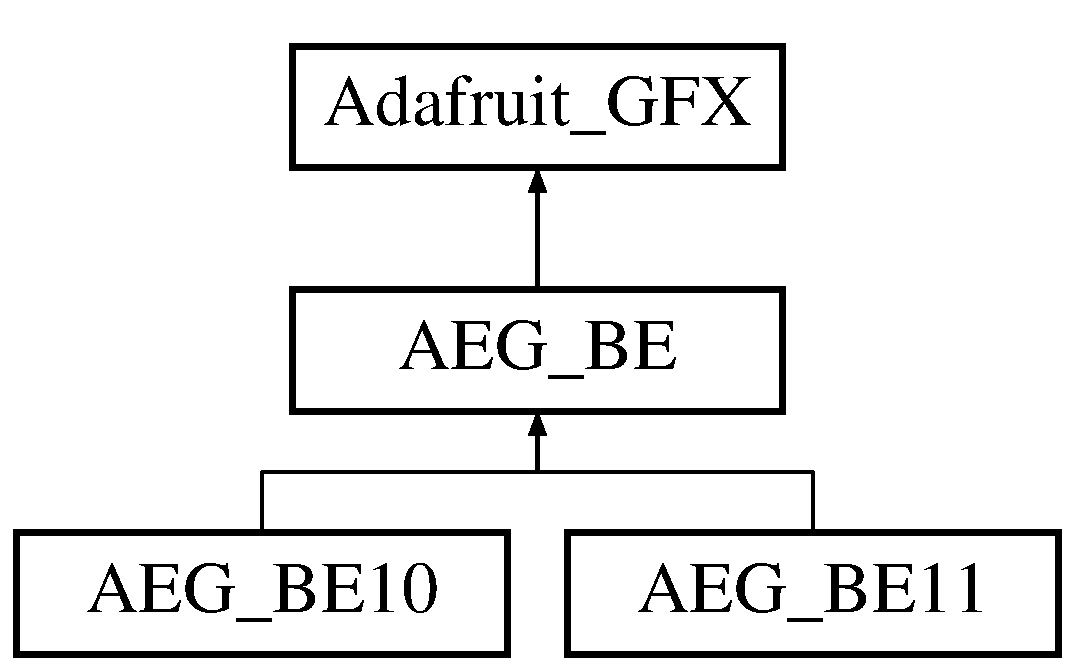
\includegraphics[height=3.000000cm]{class_a_e_g___b_e}
\end{center}
\end{figure}
\subsection*{Public Member Functions}
\begin{DoxyCompactItemize}
\item 
\mbox{\hyperlink{class_a_e_g___b_e_a85bd3c991a670cf65ed70bca2af49413}{A\+E\+G\+\_\+\+BE}} (uint8\+\_\+t, uint8\+\_\+t, uint8\+\_\+t, uint8\+\_\+t, uint8\+\_\+t)
\begin{DoxyCompactList}\small\item\em Initializes pins, buffer and other functions. \end{DoxyCompactList}\item 
void \mbox{\hyperlink{class_a_e_g___b_e_aa8755698903c6e198ca1a07788541d1a}{enable}} (void)
\item 
void \mbox{\hyperlink{class_a_e_g___b_e_a340ce74a24ba0dc26c05519a7f865f3c}{disable}} (void)
\item 
void \mbox{\hyperlink{class_a_e_g___b_e_a1256522fd3165e2894b59fee10eab621}{draw\+Pixel}} (int16\+\_\+t, int16\+\_\+t, uint16\+\_\+t)
\item 
void \mbox{\hyperlink{class_a_e_g___b_e_a26979ef08f0e328d092fecb132da511b}{fill\+Screen}} (uint16\+\_\+t)
\item 
void \mbox{\hyperlink{class_a_e_g___b_e_a01f3830d43086806b1e58a4401268d40}{display}} (void)
\end{DoxyCompactItemize}


\subsection{Detailed Description}
Display driver for various L\+CD produced by A\+EG (B\+M\+G$\vert$\+M\+IS) 

This driver supports different types of L\+C\+Ds with 40 bit shift registers (C\+OG). Currently officially supported are B\+E10 (29x24px) and B\+E11 (39x24px). Pinout of these displays is as following (starting from inside the L\+CD)\+:

1 \mbox{[}input\mbox{]} D\+A\+TA

2 \mbox{[}power\mbox{]} 5V

3 \mbox{[}power\mbox{]} 10V

4 \mbox{[}power\mbox{]} G\+ND

5 \mbox{[}input\mbox{]} E\+N\+A\+B\+LE

6 \mbox{[}input\mbox{]} L\+CD C\+L\+O\+CK

7 \mbox{[}input\mbox{]} L\+A\+T\+CH

8 \mbox{[}input\mbox{]} D\+A\+TA C\+L\+O\+CK

9 \mbox{[}output\mbox{]} D\+A\+TA 

\subsection{Constructor \& Destructor Documentation}
\mbox{\Hypertarget{class_a_e_g___b_e_a85bd3c991a670cf65ed70bca2af49413}\label{class_a_e_g___b_e_a85bd3c991a670cf65ed70bca2af49413}} 
\index{A\+E\+G\+\_\+\+BE@{A\+E\+G\+\_\+\+BE}!A\+E\+G\+\_\+\+BE@{A\+E\+G\+\_\+\+BE}}
\index{A\+E\+G\+\_\+\+BE@{A\+E\+G\+\_\+\+BE}!A\+E\+G\+\_\+\+BE@{A\+E\+G\+\_\+\+BE}}
\subsubsection{\texorpdfstring{A\+E\+G\+\_\+\+B\+E()}{AEG\_BE()}}
{\footnotesize\ttfamily A\+E\+G\+\_\+\+B\+E\+::\+A\+E\+G\+\_\+\+BE (\begin{DoxyParamCaption}\item[{uint8\+\_\+t}]{panels,  }\item[{uint8\+\_\+t}]{latch,  }\item[{uint8\+\_\+t}]{enable,  }\item[{uint8\+\_\+t}]{panelwidth,  }\item[{uint8\+\_\+t}]{registers }\end{DoxyParamCaption})}



Initializes pins, buffer and other functions. 

Constructor sets pin 3 to output 122 Hz for L\+CD clock, and latch/enable as outputs. M\+O\+SI and S\+CK are used for fast S\+PI transmission to the shift registers at 1 M\+Hz.


\begin{DoxyParams}{Parameters}
{\em panels} & Number of daisychained panels \\
\hline
{\em latch} & Latch Pin on Arduino \\
\hline
{\em enable} & Enable pin on Arduino \\
\hline
{\em panelwidth} & Pixels in width on a single panel \\
\hline
{\em registers} & Number of 40 bit shift registers in one row (top/bottom half) \\
\hline
\end{DoxyParams}


\subsection{Member Function Documentation}
\mbox{\Hypertarget{class_a_e_g___b_e_a340ce74a24ba0dc26c05519a7f865f3c}\label{class_a_e_g___b_e_a340ce74a24ba0dc26c05519a7f865f3c}} 
\index{A\+E\+G\+\_\+\+BE@{A\+E\+G\+\_\+\+BE}!disable@{disable}}
\index{disable@{disable}!A\+E\+G\+\_\+\+BE@{A\+E\+G\+\_\+\+BE}}
\subsubsection{\texorpdfstring{disable()}{disable()}}
{\footnotesize\ttfamily void A\+E\+G\+\_\+\+B\+E\+::disable (\begin{DoxyParamCaption}\item[{void}]{ }\end{DoxyParamCaption})}

Disables output of values in registers \mbox{\Hypertarget{class_a_e_g___b_e_a01f3830d43086806b1e58a4401268d40}\label{class_a_e_g___b_e_a01f3830d43086806b1e58a4401268d40}} 
\index{A\+E\+G\+\_\+\+BE@{A\+E\+G\+\_\+\+BE}!display@{display}}
\index{display@{display}!A\+E\+G\+\_\+\+BE@{A\+E\+G\+\_\+\+BE}}
\subsubsection{\texorpdfstring{display()}{display()}}
{\footnotesize\ttfamily void A\+E\+G\+\_\+\+B\+E\+::display (\begin{DoxyParamCaption}\item[{void}]{ }\end{DoxyParamCaption})}

Outputs buffer to display at 1 M\+Hz \mbox{\Hypertarget{class_a_e_g___b_e_a1256522fd3165e2894b59fee10eab621}\label{class_a_e_g___b_e_a1256522fd3165e2894b59fee10eab621}} 
\index{A\+E\+G\+\_\+\+BE@{A\+E\+G\+\_\+\+BE}!draw\+Pixel@{draw\+Pixel}}
\index{draw\+Pixel@{draw\+Pixel}!A\+E\+G\+\_\+\+BE@{A\+E\+G\+\_\+\+BE}}
\subsubsection{\texorpdfstring{draw\+Pixel()}{drawPixel()}}
{\footnotesize\ttfamily void A\+E\+G\+\_\+\+B\+E\+::draw\+Pixel (\begin{DoxyParamCaption}\item[{int16\+\_\+t}]{x,  }\item[{int16\+\_\+t}]{y,  }\item[{uint16\+\_\+t}]{color }\end{DoxyParamCaption})}

Draws pixel to buffer on corresponding position 
\begin{DoxyParams}{Parameters}
{\em x} & Position on x axis, starting with 0=left \\
\hline
{\em y} & Position on y axis, starting with 0=top \\
\hline
{\em color} & W\+H\+I\+TE or B\+L\+A\+CK \\
\hline
\end{DoxyParams}
\mbox{\Hypertarget{class_a_e_g___b_e_aa8755698903c6e198ca1a07788541d1a}\label{class_a_e_g___b_e_aa8755698903c6e198ca1a07788541d1a}} 
\index{A\+E\+G\+\_\+\+BE@{A\+E\+G\+\_\+\+BE}!enable@{enable}}
\index{enable@{enable}!A\+E\+G\+\_\+\+BE@{A\+E\+G\+\_\+\+BE}}
\subsubsection{\texorpdfstring{enable()}{enable()}}
{\footnotesize\ttfamily void A\+E\+G\+\_\+\+B\+E\+::enable (\begin{DoxyParamCaption}\item[{void}]{ }\end{DoxyParamCaption})}

Enables output of values in registers \mbox{\Hypertarget{class_a_e_g___b_e_a26979ef08f0e328d092fecb132da511b}\label{class_a_e_g___b_e_a26979ef08f0e328d092fecb132da511b}} 
\index{A\+E\+G\+\_\+\+BE@{A\+E\+G\+\_\+\+BE}!fill\+Screen@{fill\+Screen}}
\index{fill\+Screen@{fill\+Screen}!A\+E\+G\+\_\+\+BE@{A\+E\+G\+\_\+\+BE}}
\subsubsection{\texorpdfstring{fill\+Screen()}{fillScreen()}}
{\footnotesize\ttfamily void A\+E\+G\+\_\+\+B\+E\+::fill\+Screen (\begin{DoxyParamCaption}\item[{uint16\+\_\+t}]{color }\end{DoxyParamCaption})}

Fills the buffer the fastest way without touching invalid bits 
\begin{DoxyParams}{Parameters}
{\em color} & W\+H\+I\+TE or B\+L\+A\+CK \\
\hline
\end{DoxyParams}


The documentation for this class was generated from the following files\+:\begin{DoxyCompactItemize}
\item 
A\+E\+G\+\_\+\+B\+E.\+h\item 
A\+E\+G\+\_\+\+B\+E.\+cpp\end{DoxyCompactItemize}

\hypertarget{class_a_e_g___b_e10}{}\section{A\+E\+G\+\_\+\+B\+E10 Class Reference}
\label{class_a_e_g___b_e10}\index{A\+E\+G\+\_\+\+B\+E10@{A\+E\+G\+\_\+\+B\+E10}}


Alias constructor for B\+E10 displays.  




{\ttfamily \#include $<$A\+E\+G\+\_\+\+B\+E.\+h$>$}

Inheritance diagram for A\+E\+G\+\_\+\+B\+E10\+:\begin{figure}[H]
\begin{center}
\leavevmode
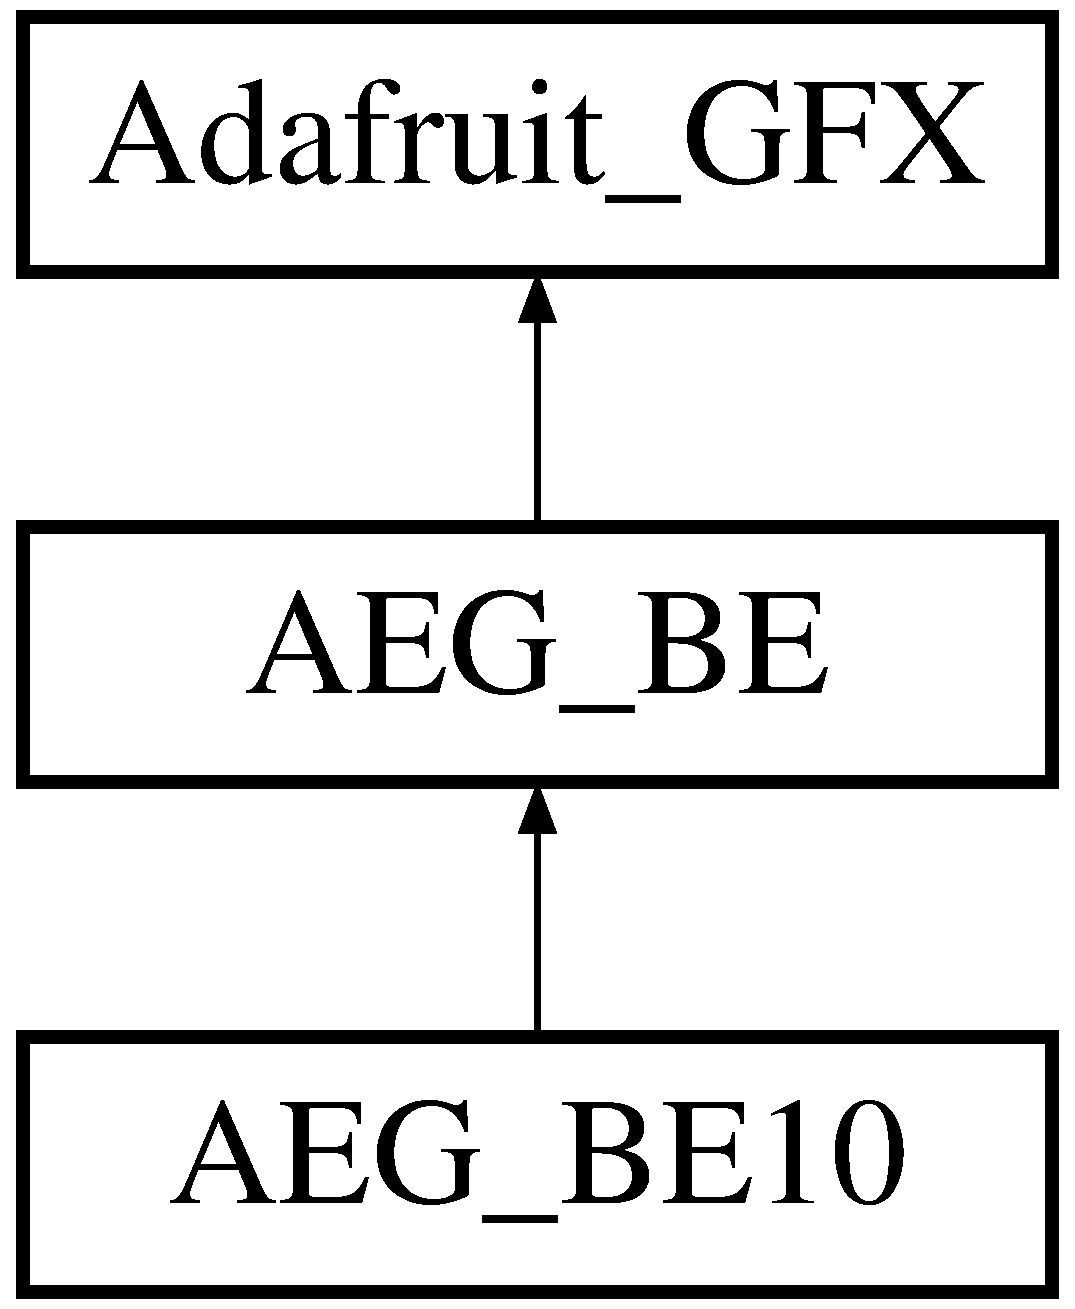
\includegraphics[height=3.000000cm]{class_a_e_g___b_e10}
\end{center}
\end{figure}
\subsection*{Public Member Functions}
\begin{DoxyCompactItemize}
\item 
\hyperlink{class_a_e_g___b_e10_af406607c342a0afffbc7991e32848552}{A\+E\+G\+\_\+\+B\+E10} (uint8\+\_\+t, uint8\+\_\+t, uint8\+\_\+t)
\begin{DoxyCompactList}\small\item\em Initializes a {\ttfamily \hyperlink{class_a_e_g___b_e}{A\+E\+G\+\_\+\+BE}} object. \end{DoxyCompactList}\end{DoxyCompactItemize}


\subsection{Detailed Description}
Alias constructor for B\+E10 displays. 

\begin{DoxySeeAlso}{See also}
\hyperlink{class_a_e_g___b_e}{A\+E\+G\+\_\+\+BE} 
\end{DoxySeeAlso}


\subsection{Constructor \& Destructor Documentation}
\mbox{\Hypertarget{class_a_e_g___b_e10_af406607c342a0afffbc7991e32848552}\label{class_a_e_g___b_e10_af406607c342a0afffbc7991e32848552}} 
\index{A\+E\+G\+\_\+\+B\+E10@{A\+E\+G\+\_\+\+B\+E10}!A\+E\+G\+\_\+\+B\+E10@{A\+E\+G\+\_\+\+B\+E10}}
\index{A\+E\+G\+\_\+\+B\+E10@{A\+E\+G\+\_\+\+B\+E10}!A\+E\+G\+\_\+\+B\+E10@{A\+E\+G\+\_\+\+B\+E10}}
\subsubsection{\texorpdfstring{A\+E\+G\+\_\+\+B\+E10()}{AEG\_BE10()}}
{\footnotesize\ttfamily A\+E\+G\+\_\+\+B\+E10\+::\+A\+E\+G\+\_\+\+B\+E10 (\begin{DoxyParamCaption}\item[{uint8\+\_\+t}]{panels,  }\item[{uint8\+\_\+t}]{latch,  }\item[{uint8\+\_\+t}]{enable }\end{DoxyParamCaption})}



Initializes a {\ttfamily \hyperlink{class_a_e_g___b_e}{A\+E\+G\+\_\+\+BE}} object. 

A\+EG BE L\+CD Library \begin{DoxyAuthor}{Author}
Luca Zimmermann 
\end{DoxyAuthor}
\begin{DoxyVersion}{Version}
1.\+1 18.\+12.\+2017 
\end{DoxyVersion}

\begin{DoxyParams}{Parameters}
{\em panels} & Number of daisychained panels \\
\hline
{\em latch} & Latch Pin on Arduino \\
\hline
{\em enable} & Enable pin on Arduino \\
\hline
\end{DoxyParams}


The documentation for this class was generated from the following files\+:\begin{DoxyCompactItemize}
\item 
A\+E\+G\+\_\+\+B\+E.\+h\item 
A\+E\+G\+\_\+\+B\+E.\+cpp\end{DoxyCompactItemize}

\hypertarget{class_a_e_g___b_e11}{}\section{A\+E\+G\+\_\+\+B\+E11 Class Reference}
\label{class_a_e_g___b_e11}\index{A\+E\+G\+\_\+\+B\+E11@{A\+E\+G\+\_\+\+B\+E11}}


Alias constructor for B\+E11 displays.  




{\ttfamily \#include $<$A\+E\+G\+\_\+\+B\+E.\+h$>$}

Inheritance diagram for A\+E\+G\+\_\+\+B\+E11\+:\begin{figure}[H]
\begin{center}
\leavevmode
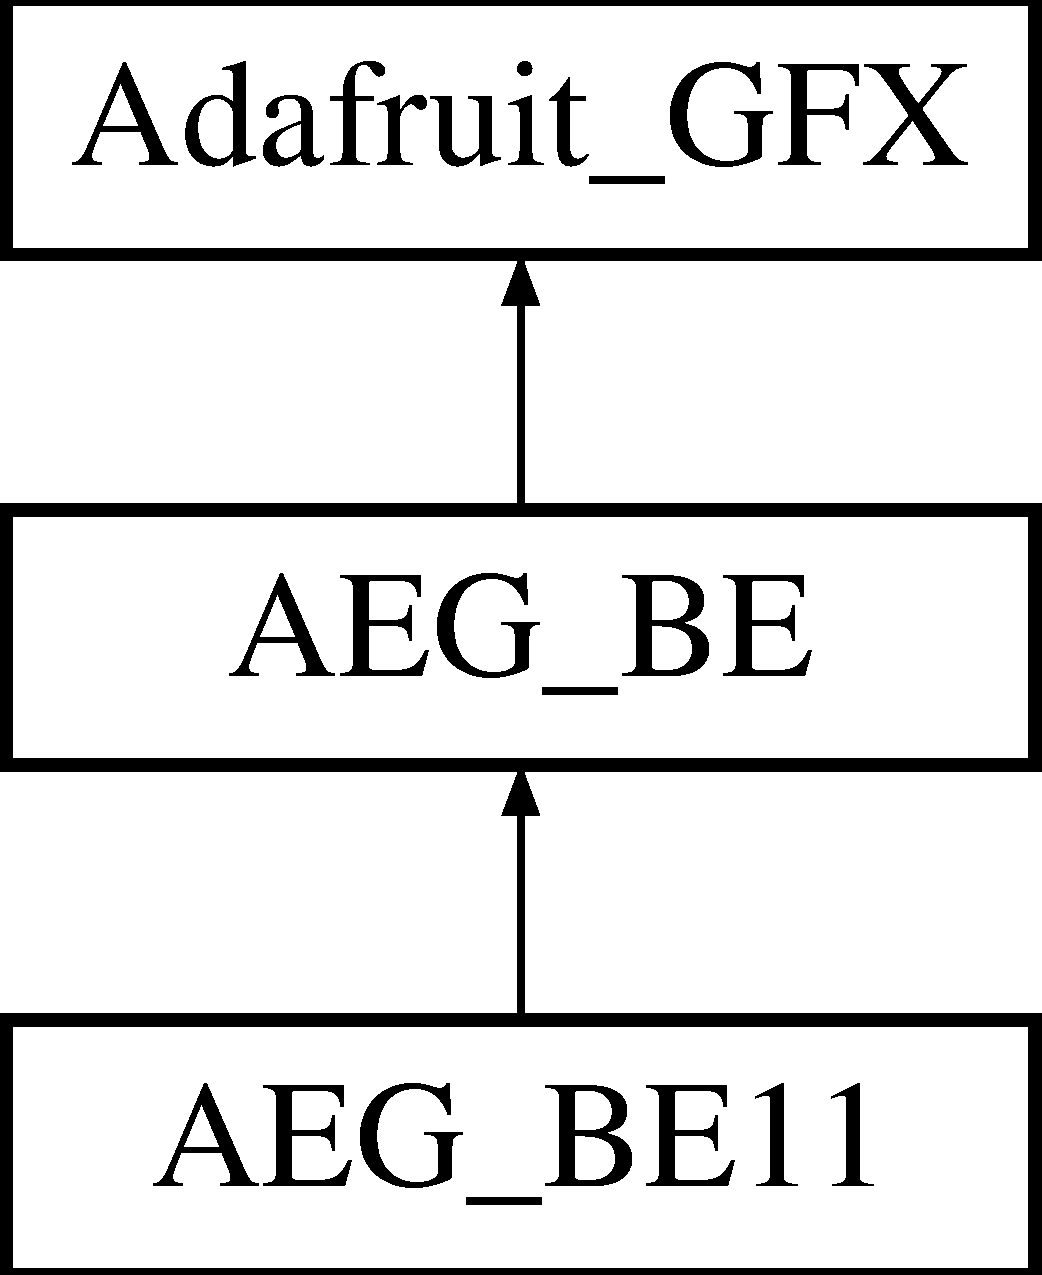
\includegraphics[height=3.000000cm]{class_a_e_g___b_e11}
\end{center}
\end{figure}
\subsection*{Public Member Functions}
\begin{DoxyCompactItemize}
\item 
\hyperlink{class_a_e_g___b_e11_addb3a2e7c180491a65374fdef38f67da}{A\+E\+G\+\_\+\+B\+E11} (uint8\+\_\+t, uint8\+\_\+t, uint8\+\_\+t)
\begin{DoxyCompactList}\small\item\em Initializes a {\ttfamily \hyperlink{class_a_e_g___b_e}{A\+E\+G\+\_\+\+BE}} object. \end{DoxyCompactList}\end{DoxyCompactItemize}


\subsection{Detailed Description}
Alias constructor for B\+E11 displays. 

\begin{DoxySeeAlso}{See also}
\hyperlink{class_a_e_g___b_e}{A\+E\+G\+\_\+\+BE} 
\end{DoxySeeAlso}


\subsection{Constructor \& Destructor Documentation}
\mbox{\Hypertarget{class_a_e_g___b_e11_addb3a2e7c180491a65374fdef38f67da}\label{class_a_e_g___b_e11_addb3a2e7c180491a65374fdef38f67da}} 
\index{A\+E\+G\+\_\+\+B\+E11@{A\+E\+G\+\_\+\+B\+E11}!A\+E\+G\+\_\+\+B\+E11@{A\+E\+G\+\_\+\+B\+E11}}
\index{A\+E\+G\+\_\+\+B\+E11@{A\+E\+G\+\_\+\+B\+E11}!A\+E\+G\+\_\+\+B\+E11@{A\+E\+G\+\_\+\+B\+E11}}
\subsubsection{\texorpdfstring{A\+E\+G\+\_\+\+B\+E11()}{AEG\_BE11()}}
{\footnotesize\ttfamily A\+E\+G\+\_\+\+B\+E11\+::\+A\+E\+G\+\_\+\+B\+E11 (\begin{DoxyParamCaption}\item[{uint8\+\_\+t}]{panels,  }\item[{uint8\+\_\+t}]{latch,  }\item[{uint8\+\_\+t}]{enable }\end{DoxyParamCaption})}



Initializes a {\ttfamily \hyperlink{class_a_e_g___b_e}{A\+E\+G\+\_\+\+BE}} object. 


\begin{DoxyParams}{Parameters}
{\em panels} & Number of daisychained panels \\
\hline
{\em latch} & Latch Pin on Arduino \\
\hline
{\em enable} & Enable pin on Arduino \\
\hline
\end{DoxyParams}


The documentation for this class was generated from the following files\+:\begin{DoxyCompactItemize}
\item 
A\+E\+G\+\_\+\+B\+E.\+h\item 
A\+E\+G\+\_\+\+B\+E.\+cpp\end{DoxyCompactItemize}

%--- End generated contents ---

% Index
\backmatter
\newpage
\phantomsection
\clearemptydoublepage
\addcontentsline{toc}{chapter}{Index}
\printindex

\end{document}
